\chapter{Конструкторский раздел}
\section{База данных}
Рассмотрим процесс перехода от ER-диаграммы (рис.~\ref{fig:er}) к схеме базы данных (рис.~\ref{fig:database}):
\begin{enumerate}
  \item В силу регламентированности структуры данных имеет смысл использовать реляционную схему базы данных;
  \item Сущность <<слово>> естественным образом переходит в таблицу \verb|word|, причём без сохранения производных атрибутов (IDF), в силу тривиальности их расчёта;
  \item Сущность <<страница>> переходит в две таблицы: \verb|page| и \verb|indexed|, так как все атрибуты кроме <<URL>> и <<ключа>> могут быть получены только после разбора страницы, а <<URL>> и <<ключ>> получены и из ссылок на другие страницы. На практике количество неразобранных страниц на несколько порядков больше проиндексированных, а значит использование только одной таблице ведёт к неоправданному расходу памяти;
  \item Связь многие-ко-многим <<содержит>> переходит в таблицу \verb|location| вместе с непроизводными атрибутами;
  \item Связь многие-ко-многим <<ссылается на>> переходит в таблицы \verb|link| и \verb|linkword|. Данная денормализация вызвана необходимостью поисковой оптимизации (см.~\ref{sssec:optimization});
\end{enumerate}

\begin{figure}[h]
  \centering
  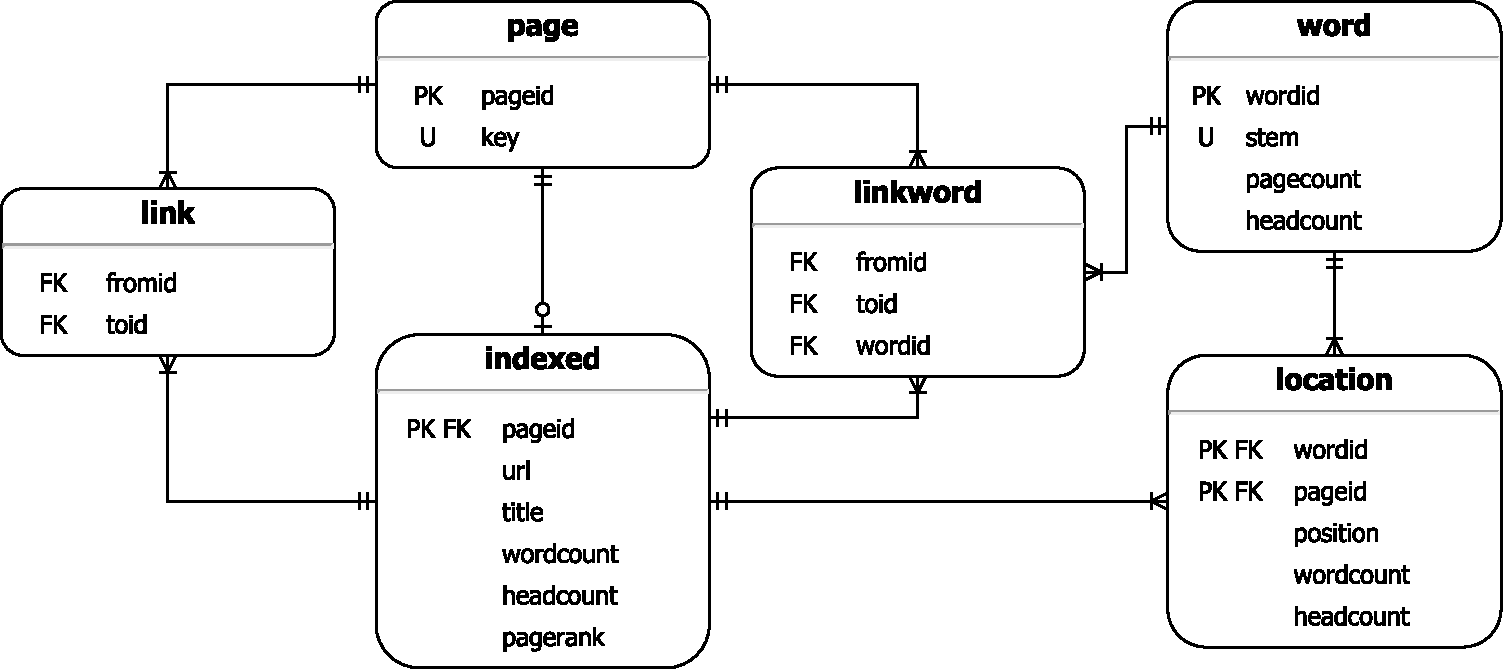
\includegraphics[width=\textwidth]{database.pdf}
  \caption{Схема базы данных.}
  \label{fig:database}
\end{figure}

Рассмотрим подробнее каждую таблицу:

\begin{definition}{\texttt{page(\underline{pageid}, key)}}
  Таблица содержит информацию о страницах, которые когда-либо встречались поисковым роботом. Сюда входят как посещённые страницы, так и ещё не обработанные страницы, ссылка на которые когда-либо встречалась. Поле \verb|key| содержит уникальный ключ страницы, получающийся в результате агрессивной нормализации URL (см. раздел~\ref{sssec:url-normalization}).
\end{definition}

\begin{definition}{\texttt{word(\underline{wordid}, stem, pagecount, headcount)}}
  Информация о словах, когда либо индексировавшихся роботом. Поле \verb|stem| содержит уникальную основу слова (см. раздел~\ref{sssec:stemming}), \verb|pagecount|~--- количество проиндексированных страниц, содержащих данное слово в любой форме, а \verb|headcount|~--- количество проиндексированных страниц, в заголовках которых встретилось данное слово (см. раздел~\ref{sssec:tf-idf}).
\end{definition}

\begin{definition}{\texttt{indexed(\underline{pageid}, url, title, wordcount, headcount, pagerank)}}
  Таблица всех проиндексированных страниц, содержащая URL-адрес \verb|url|, заголовок страницы \verb|title|, количество слов в документе \verb|wordcount|, количество слов в заголовках документа \verb|headcount| и ранг страницы \verb|pagerank| (см. раздел~\ref{sssec:pagerank}). Заголовок страницы не обязательно будет совпадать со значением \verb|<title>|, особенно если последнего нет или он пустой. URL хранится в безопасно нормализованной форме (см. раздел~\ref{sssec:url-normalization}), чтобы пользователь мог воспользоваться оригинальным URL.
\end{definition}

\begin{definition}{\texttt{location(\underline{wordid, pageid}, position, wordcount, headcount)}}
  Инвертированный индекс, содержащий информацию о каждом слове на странице: позиция первого вхождения \verb|position| (см. раздел~\ref{sssec:position}), количество вхождений в текст \verb|wordcount| и в заголовки \verb|headcount| (см. раздел~\ref{sssec:bm25}).
\end{definition}

\begin{definition}{\texttt{link(fromid, toid)}}
  Таблица ссылок, связывающая однозначно проиндексированную страницу с идентификатором \verb|fromid| и страницу (необязательно проиндексированную) с идентификатором \verb|toid|. Не содержит ссылок с атрибутом \verb|rel="nofollow"| (см. раздел~\ref{sssec:links}).
\end{definition}

\begin{definition}{\texttt{linkword(fromid, toid, wordid)}}
  Таблица слов в ссылках между \verb|fromid| и \verb|toid|. Совокупность пар (\verb|fromid|, \verb|toid|) является подмножеством отношения \verb|link|, однако замена этой пары на идентификатор \verb|link| ведёт к усложнению поиска и невозможности некоторых оптимизаций (см. раздел~\ref{sssec:optimization}). Не содержит ссылок с атрибутом \verb|rel="nofollow"| и не относящихся к основному содержимому (см. раздел~\ref{sssec:readability}).
\end{definition}


\section{Поисковой робот}
\subsection{Архитектура робота}
Упрощённо процесс работы такого робота состоит из следующих этапов (рис. \ref{fig:crawler}):
\begin{enumerate}
  \item Всё начинается с того, что пользователь роботом \framebox{1} добавляет в очередь \framebox{2} какой-то начальный набор адресов, с которого и начнётся обход;
  \item Загрузчик страниц \framebox{3} получает из очереди \framebox{2} очередной адрес и производит соответствующий HTTP-запрос через сеть Интернет \framebox{4}. Чтобы избежать DNS-запросов перед загрузкой каждой страницы, IP-адрес домена кешируется;
  \item В случае успешного ответа загрузчик \framebox{3} передаёт страницу в экстрактор информации \framebox{4};
  \item Экстрактор информации \framebox{5} извлекает из страницы ссылки и полезную текстовую информацию. После чего ссылки добавляются в очередь \framebox{2}, а текстовой документ отправляется в индексатор \framebox{6};
  \item Индексатор \framebox{6} подготавливает документ и формирует запросы на сохранение в базу данных \framebox{7}.
\end{enumerate}

\begin{figure}[h]
  \centering
  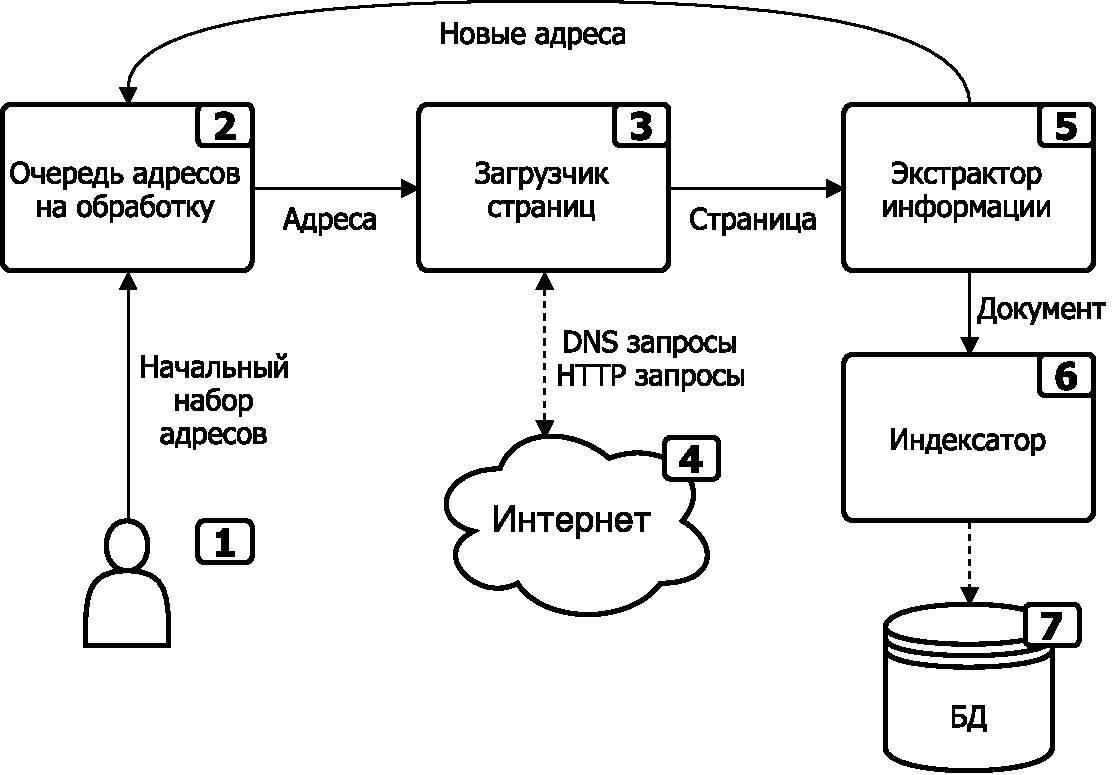
\includegraphics[width=\linewidth]{crawler.pdf}
  \caption{Архитектура поискового робота.}
  \label{fig:crawler}
\end{figure}

Несколько уточнений по работе поискового робота:
\begin{enumerate}
  \item Связь между компонентами осуществляется асинхронно;
  \item Используется несколько загрузчиков страниц, работающих параллельно;
  \item Очередь адресов представляет собой комплексную структуру (о чём далее).
\end{enumerate}


\subsection{Очередь адресов}
Адреса, принадлежащие одному домену имеют общую информацию, такую как набор правил, заданного в \verb|robots.txt| (см. раздел~\ref{ssec:robotstxt}) и IP-адрес, кеширование которого позволяет уменьшить количество DNS-запросов. Поэтому необходимо группировать страницы в домены, которые и будут содержаться в очереди.

Используется очередь доменов с приоритетом, основанная на бинарной куче. В качестве приоритета задаётся время пробуждения, которое получается как сумма времени предыдущего запроса и времени, необходимого для ожидания, которое может быть получено либо из \verb|robots.txt|, если владелец сайта явно ограничил частоту запросов, либо из соображений длительности отклика сервера: при сильных нагрузках сервера отвечают значительно реже.

Удаление доменов из очереди происходит после определённого (наперёд заданного) времени бездействия в порядке обычной обработки очереди.

Кроме того, внутри каждого домена существует очередь с приоритетом из страниц. Здесь, в качестве приоритета приняты штрафные очки страницы, которые суммируются из следующих факторов:
\begin{itemize}
  \item Была ли ссылка на эту страницу в основном содержимом;
  \item Содержала ли ссылка текст;
  \item Текущая глубина обхода;
  \item Содержала ли ссылка атрибут \verb|rel="nofollow"| (или был он добавлен в результате обработки динамической ссылки, см. раздел~\ref{sssec:url-normalization});
\end{itemize}


\section{Постобработка}
После сбора коллекции документов необходима некоторая обработка данных для вычисления PageRank (см. раздел~\ref{sssec:pagerank}) и BM25 (см. раздел~\ref{sssec:bm25}).


\subsection{Вычисление PageRank}
Для правильного вычисления ранга страницы нужно иметь сеть, обладающую только внутренними ссылками, то есть такую, где все ссылки указывают только на проиндексированные страницы. Для этого создаётся и заполняется временная таблица \verb|inboundlink| (рис.~\ref{fig:inboundlink}), основываясь на таблице \verb|link| (листинг~\ref{lst:inboundlink}).
\begin{figure}[h]
  \centering
  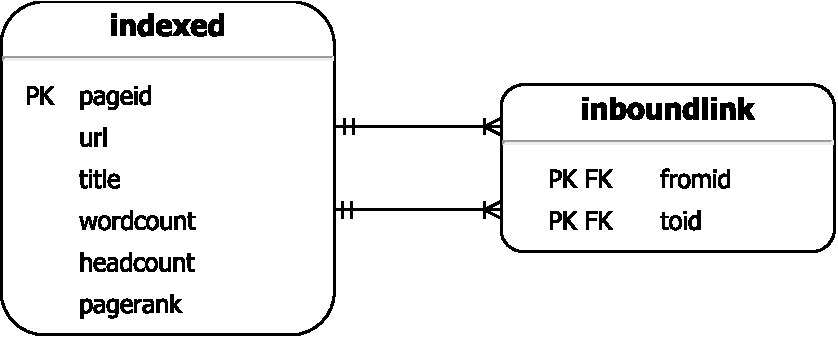
\includegraphics[width=.7\textwidth]{inboundlink.pdf}
  \caption{Концептуальная ER-диаграмма связей внутри коллекции.}
  \label{fig:inboundlink}
\end{figure}

\begin{lstlisting}[language=sqlite, caption=Выборка внутренних для коллекции ссылок., label=lst:inboundlink]
select fromid, toid
from indexed ifr, indexed ito join link
on fromid = ifr.pageid and toid = ito.pageid;
\end{lstlisting}

После чего можно приступать непосредственно к вычислению PageRank. Сначала необходимо задать базовый ранг страницы, например 1, и подсчитать количество ссылок на странице (листинг~\ref{lst:pr-initialization}).
\begin{lstlisting}[language=sqlite, caption=Инициализация процесса вычисления PageRank., label=lst:pr-initialization]
select pageid, count(toid), 1.
from indexed left join inboundlink on pageid = fromid
group by pageid;
\end{lstlisting}

Значения на очередной итерации могут быть вычислены, используя~\ref{eq:pagerank}, как показано на листинге~\ref{lst:pr-iteration}. Функция \verb|total| эквивалентна функции \verb|sum| из стандарта SQL, за исключением того, что на пустой выборке возвращает \verb|0|, а не \verb|NULL|.
\begin{lstlisting}[language=sqlite, caption=Итерация процесса вычисления PageRank., label=lst:pr-iteration]
select src.pageid, src.linkcount, .15 + .85 * total(fr.pagerank/fr.linkcount)
from src left join inboundlink on src.pageid = toid
         left join src fr on fr.pageid = fromid
group by src.pageid;
\end{lstlisting}


\subsection{Общая информация}
Помимо ранга страницы необходимо найти некоторую общую информацию, такую как общее количество документов в коллекции, средняя длина в словах документа и средняя длина в словах в заголовках документа (листинг~\ref{lst:info}).
\begin{lstlisting}[language=sqlite, caption=Нахождение общей информации., label=lst:info]
select count(*), avg(wordcount), avg(headcount) from indexed;
\end{lstlisting}

Кроме того, самое время указать СУБД на необходимость заново проанализировать базу данных (команда \verb|analyze|), что может быть полезно для внутренней оптимизации запросов к базе данных.


\section{Поиск}
Для получения списка релевантных документов и всей необходимой для их ранжирования информации формируется один большой запрос, зависящий от количества запрашиваемых слов и их идентификаторов. Данный запрос является узким местом при поиске и должен быть максимально оптимизирован.

Пример упрощённого сформированного запроса двух слов с идентификаторами 42 и 146 представлен на листинге~\ref{lst:query}.
\begin{lstlisting}[language=sqlite, caption=Запрос релевантных документов., label=lst:query]
select
  idx.pageid,                 -- идентификатор страницы
  idx.wordcount,              -- количество слов на странице
  idx.headcount,              -- количество слов в заголовках страницы
  idx.pagerank,               -- ранг страницы
  total(fromidx.pagerank),    -- реферальный ранг страницы
  l0.position + l1.position,  -- близость слов к началу
  l0.wordcount, l0.headcount, -- частотность первого слова
  l1.wordcount, l1.headcount  -- частотность второго слова

from location l0
join location l1 using (pageid)
join indexed idx using (pageid)
left join linkword lw on lw.wordid in (42, 146)
                     and idx.pageid = toid
left join indexed fromidx on fromidx.pageid = fromid

where l0.wordid = 42 and l1.wordid = 146
group by l0.pageid
\end{lstlisting}

В данном запросе в результирующий набор попадают страницы, которые обладают всеми запрошенными словами. Кроме того, для каждой страницы просчитывается суммарный реферальный ранг страницы.


\subsection{Оптимизация запроса}
Так как данный запрос является ядром поиска и при этом наиболее узким местом, то необходимо максимально оптимизировать его. Рассмотрим несколько техник.


\subsubsection{Оптимизация перебора} \label{sssec:optimization}
Рассмотрим план выполнения запроса (листинг~\ref{lst:query}) и попробуем оптимизировать его (листинг~\ref{lst:bad-plan}).
\begin{lstlisting}[language=sql-explain, caption=Неоптимальный план выполнения запроса., label=lst:bad-plan]
SEARCH TABLE location AS l0 USING PRIMARY KEY (wordid=?)
SEARCH TABLE location AS l1 USING PRIMARY KEY (wordid=? AND pageid=?)
SEARCH TABLE indexed AS idx USING PRIMARY KEY (pageid=?)
SCAN TABLE linkword AS lw
SEARCH TABLE indexed AS fromidx USING PRIMARY KEY (pageid=?)
\end{lstlisting}

\verb|SCAN TABLE| в плане запроса указывает на полное сканирование таблицы \verb|linkword|. Для ускорения поиска требуется создать дополнительный индекс (листинг~\ref{lst:index}).
\begin{lstlisting}[language=sqlite, caption=Создание индекса., label=lst:index]
create index wordidtoididx on linkword(wordid, toid);
\end{lstlisting}

Теперь запрос будет выполнен максимально оптимизированным образом (листинг~\ref{lst:good-plan}): со сложностью $O(\log n)$ вместо $O(n)$ при поиске по таблице \verb|linkword| в силу использования B/B+-деревьев внутри движка запросов СУБД.
\begin{lstlisting}[language=sql-explain, caption=Оптимальный план выполнения запроса., label=lst:good-plan]
SEARCH TABLE location AS l0 USING PRIMARY KEY (wordid=?)
SEARCH TABLE location AS l1 USING PRIMARY KEY (wordid=? AND pageid=?)
SEARCH TABLE indexed AS idx USING PRIMARY KEY (pageid=?)
SEARCH TABLE linkword AS lw USING INDEX wordidtoididx (wordid=? AND toid=?)
EXECUTE LIST SUBQUERY 1
SEARCH TABLE indexed AS fromidx USING PRIMARY KEY (pageid=?)
\end{lstlisting}


\subsubsection{Предварительная сортировка слов}
При выполнения запроса (листинг~\ref{lst:query}) большую роль играет последовательность слов. Действительно, если первое слово встречается чаще, чем последующие, то интерпретатору запроса придётся проверить больше документов. Сортировка слов по возрастанию их частоты позволяет отбрасывать нерелевантные документы раньше.


\section{Сервер и поисковая страница}
Для того, чтобы пользователь смог воспользоваться графическим интерфейсом поисковой системы, необходим работающий веб-сервер, который отдаст поисковую страницу в ответ на запрос. Поскольку запросы могут выполняться продолжительное время, веб-сервер работает в асинхронном режиме, а все запросы к базе данных осуществляются в отдельном потоке.

Поисковый запрос передаётся методом \verb|GET| с передачей параметров запроса (сам текст запроса и количество страниц, которые следует пропустить после ранжирования). Чтобы текст запроса был передан без искажений производится кодирование текста как компонента URI, путём замены всех символов, за исключением латинских букв, цифр и знаков <<->>, <<\_>>, <<.>>, <<!>>, <<~>>, <<*>>, <<'>>, <<(>>, <<)>>. Например, пользователь может произвести запрос с текстом <<Python\&language>>, что выделит новую пару ключ-значение из-за использования амперсанда. Поэтому вместо одного параметра <<Python\&language>> будут получены два и запрос будет произведён только для <<Python>>.
